\documentclass[exercice,a4]{thedocument}%
\usepackage{texmaths-tikz}%
\usepackage[np]{numprint}%
\startdatakeys
\source{24GENMATAN1}
\BO{2026}
\cycle{4}
\competencesDuSocle{CA,RA}
\objectifsApprentissage{C4B2cd,C4B2cb,C4D2ac,C4D2ad,C4D2ae}
\motsCles{Pythagore,périmètre,aire,volume,prisme,proportionnalité,ratio}
\enddatakeys
\begin{document}%
\def\up#1{\textsuperscript{#1}}%
M. et M\up{me} Martin veulent construire une terrasse en béton dans leur
jardin. Ils souhaitent que leur terrasse ait une hauteur de $15$~cm. Les
représentations ci-dessous ne sont pas à l'échelle.

\begin{center}
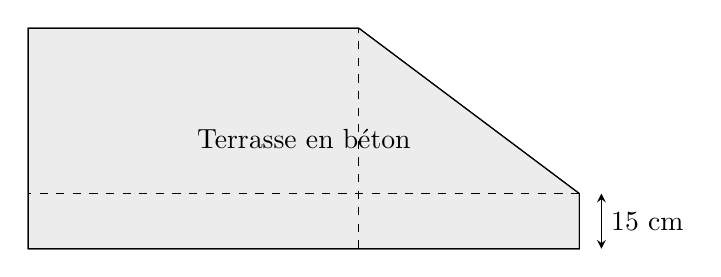
\begin{tikzpicture}[scale=.7,>=stealth]
    \draw[fill=gray!15] (0,0)--(10,0)--(10,1)--(6,4)--(0,4)--cycle;
    \draw (0,0)--(6,0)--(10,0)--(10,1)--(6,4)--(0,4)--cycle;
    \draw[dashed] (0,0)--(0,1)--(10,1) (6,0)--(6,4);
    \draw[<->] (10.4,0)--(10.4,1) node[midway,right]{15 cm};
    \node at (5,2){Terrasse en béton};
\end{tikzpicture}

\medskip
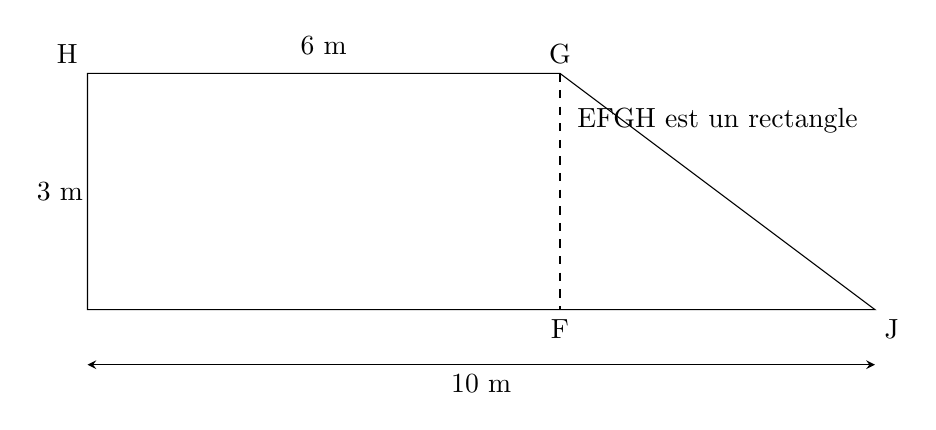
\begin{tikzpicture}[>=stealth]
    \draw (0,0)--(10,0) node[below right]{J}--(6,3) node[above]{G}
        --(0,3) node[above left]{H}--cycle;
    \draw[dashed] (6,3)--(6,0) node[below]{F};
    \draw[<->] (0,-.7)--(10,-.7) node[midway,below]{10 m};
    \node at (3,3.35){6 m};
    \node at (-.35,1.5){3 m};
    \node at (8,2.4){EFGH est un rectangle};
\end{tikzpicture}
\end{center}

\begin{enumerate}
    \item Montrer que FJ $=4$~m.
    \item Afin de pouvoir couler le béton, M. et M\up{me} Martin doivent
    délimiter la terrasse en installant des planches tout autour. Quelle
    longueur de planches doivent-ils acheter au minimum ?
    \item M. et M\up{me} Martin souhaitent réaliser $4~\mathrm{m^3}$ de béton.
    \begin{enumerate}
        \item Montrer que le volume de la terrasse est bien inférieur à
        $\np[m^3]{4}$.
        \item Sachant que pour faire $\np[m^3]{1}$ de béton, il faut
        $\np[kg]{250}$ de ciment, quelle masse de ciment doivent-ils acheter
        pour réaliser $\np[m^3]{4}$ de béton ?
        \item Dans le mélange, les masses de ciment, gravier et sable sont
        dans le ratio $2:7:5$. Déterminer, en kg, les masses de gravier et
        de sable nécessaires pour réaliser les $\np[m^3]{4}$ de béton.
    \end{enumerate}
    \item M. et M\up{me} Martin souhaitent peindre la surface supérieure de
    leur terrasse. À l'aide des documents ci-dessous, déterminer le type et
    le nombre de pots nécessaires pour effectuer ces travaux avec un coût
    minimum.
\end{enumerate}

\begin{center}
\begin{tabular}{|c|c|c|}
\hline
& Pot A & Pot B\\ \hline
Contenance (en litres) & 5 & 10\\ \hline
Prix (en euros) & 79,90 & 129,90\\ \hline
\end{tabular}

\medskip
\fbox{\begin{minipage}{.7\linewidth}
\textbf{Offre du mois :} moins 50\,\% sur le deuxième article identique.
\end{minipage}}

\medskip
\fbox{\begin{minipage}{.7\linewidth}
\textbf{Rendement :} deux couches de peinture sont nécessaires et un litre
de peinture permet de réaliser une couche de $\np[m^2]{5}$.
\end{minipage}}
\end{center}
\showthesource
\end{document}
